\newpage
\chapter{Ecuaciones y sistemas}

\begin{definicion}[Ecuación Diferencial y solución]
    Una ecuación diferencial viene dada por una función
    \Func{\Phi}{D\subseteq \mathbb{R}^3}{\mathbb{R}}{(t,x,y)}{\Phi(t,x,y)}
    \textbf{continua} donde $D$ es un \textbf{abierto}\footnote{Por convenio, ya que las ecuaciones diferenciales no se comportan bien en los bordes.} \textbf{conexo}\footnote{Es lógico pensarlo, ya que estamos estudiando movimientos.} de $\mathbb{R}^3$.

\noindent
Una \textbf{solución} de dicha ecuación diferencial será una función
\Func{x}{I}{\mathbb{R}}{t}{$x(t)$}
con $I\subseteq \mathbb{R}^2$ \textbf{intervalo}\footnote{Es lógico, pues usualmente $t$ será el tiempo.} \textbf{abierto}\footnote{Pudiendo trabajar con funciones continuas en un cerrado y derivables en el abierto, evitando así por ejemplo tangentes verticales} tal que:
\begin{enumerate}[label=\roman*)]
    \item $x$ sea derivable en $I$\footnote{Necesario para poder considerar $x'(t)$ en la propia ecuación.}.
    \item $(t,x(t),x'(t)) \in D \quad\forall t\in I$\footnote{En vistas de III).}.
    \item $\Phi(t,x(t),x'(t))=0 \quad \forall t\in I$.
\end{enumerate}
\end{definicion}

\begin{ejemplo}
    Dada la ecuación diferencial:
    \begin{equation*}
        x'(t) = \dfrac{1}{x(t)}
    \end{equation*}
    y la expresión:
    \begin{equation*}
        x(t) = \sqrt{2t-38}
    \end{equation*}
    Probar que dicha expresión es solución de la ecuación diferencial.\\

    La ecuación diferencial viene dada por
    \Func{\Phi}{\mathbb{R}\times\mathbb{R}^+\times \mathbb{R}}{\mathbb{R}}{(t,x,y)}{y-\frac{1}{x}}
    \begin{itemize}
        \item Cogiendo $I = \left]19, +\infty\right[$, tenemos I).
        \item Por ser la raíz una función continua y creciente, tenemos que ${x(I) = \left]0,+\infty\right[=\mathbb{R}^+}$, de donde se cumple II).
        \item 
            \begin{equation*}
                x'(t) = \dfrac{1}{\sqrt{2t-38}} = \dfrac{1}{x(t)} \qquad \forall t\in I
            \end{equation*}
    \end{itemize}
\end{ejemplo}

\begin{notacion}
    La notación que hemos estado utilizando para las ecuaciones diferenciales no es la que usaremos a lo largo del curso:\\

    Lo que hasta ahora hemos notado y entendido por:
    \begin{equation*}
        \Phi(t,x(t),x'(t)) = 0
    \end{equation*}

    Como en el caso:
    \begin{equation*}
      x'(t) = 3x(t)  
    \end{equation*}
    Lo notaremos ahora por:
    \begin{gather*}
        \Phi(t,x,x') = 0\\
        x' = 3x
    \end{gather*}

    Que recordamos tiene por solución:
    \begin{equation*}
        x(t) = c \cdot e^{3t}, \quad c \in \mathbb{R}
    \end{equation*}
\end{notacion}

\begin{ejemplo}
    Para cierto $\lm \in \mathbb{R}$, resolver:
    \begin{enumerate}
        \item $x' = \lm x$
            \begin{equation*}
                x(t) = c \cdot e^{\lm t} \quad c \in \mathbb{R}
            \end{equation*}
        \item $x' = \lm t$
            \begin{equation*}
                x(t) = \frac{\lm}{2} t^2 + c \quad c \in \mathbb{R}
            \end{equation*}
    \end{enumerate}
\end{ejemplo}

\section{Crecimiento proporcional}


En el capítulo anterior nos preguntábamos si todas las soluciones de la ecuación $x'=\lm x$ para cierto $\lm \in \mathbb{R}$ eran de la forma
\begin{equation*}
    x(t) = c \cdot e^{\lm t} \quad c\in \mathbb{R}
\end{equation*}
Ahora daremos respuesta a dicha cuestión, comentando además utilidades de la misma ecuación.

\begin{prop}
    Dada $x(t)$, solución de $x'=\lm x$ para cierto $\lm \in \mathbb{R}$, definida en un intervalo abierto $I$, existe $c\in \mathbb{R}$ tal que
    \begin{equation*}
        x(t) = c \cdot e^{\lm t} \quad t\in I
    \end{equation*}
\end{prop}
Antes de dar paso a la demostración, observemos que si suponemos cierta la tesis:
\begin{equation*}
    x(t) = c \cdot e^{\lm t} \Longleftrightarrow  e^{-\lm t} x(t) = c \Longrightarrow \dfrac{d}{dt}(e^{-\lm t}x(t)) = 0
\end{equation*}
\begin{proof}
    Definimos la función
    \Func{f}{I}{\mathbb{R}}{t}{e^{-\lm t}x(t)}
    que es derivable por ser producto de funciones derivables.
    \begin{align*}
        \dfrac{df(t)}{dt} = \dfrac{d}{dt}(e^{-\lm t}x(t)) &= -\lm e^{-\lm t} x(t) + e^{-\lm t} x'(t)\\
                          &= -\lm e^{-\lm t}x(t) + \lm e^{-\lm t}x(t) = 0 \quad \forall t\in I
    \end{align*}
    Por ser $f$ continua y definida en un intervalo, llegamos a que es constante, luego $\exists c\in \mathbb{R} \mid f(t) = e^{-\lm t}x(t) = c \quad \forall t\in I$, de donde deducimos que:
    \begin{equation*}
        x(t) = c \cdot e^{\lm t} \quad \forall t\in I
    \end{equation*}
\end{proof}

Nos centraremos ahora en la idea intuitiva de derivada como representación de la variación de una variable dependiente para dar lugar a los siguientes dos ejemplos que nos muestran cómo surge la ecuación diferencial $x' = \lm x$ para cierto $\lm \in \mathbb{R}$ de forma natural.

\begin{ejemplo}
    Si ingresamos un capital inicial $C(0) = 100$ en un banco que nos da el 2\% anual de interés, al cabo de un año tendremos en nuestra cuenta:
    \begin{equation*}
        C(1) = C(0) + \dfrac{2}{100}C(0) = 100 + \dfrac{2}{100}\cdot 100 = 102
    \end{equation*}
Sin embargo, si acudimos a otro banco que nos ofrece la misma tasa anual de interés pero que nos realiza pagos semestrales, al cabo de un año conseguiremos reunir:
\begin{align*}
    C(\nicefrac{1}{2}) &= C(0) + \dfrac{1}{2}\dfrac{2}{100}C(0) = 100 + \dfrac{1}{2}\dfrac{2}{100}\cdot 100 = 101 \\
    C(1) &= C(\nicefrac{1}{2}) + \dfrac{1}{2}\dfrac{2}{100}C(\nicefrac{1}{2}) = 101 + \dfrac{1}{2}\dfrac{2}{100}\cdot 101 = 102.01 > 102
\end{align*}
En general, si $\Delta t$ es la fracción del año en la que se nos hacen los pagos ($\Delta t = 1$ significa que es pago anual), la fórmula es:
\begin{equation*}
    C(t+\Delta t) = C(t) + \dfrac{2}{100}\Delta t C(t)
\end{equation*}

de donde:
\begin{equation*}
    \dfrac{C(t+\Delta t) - C(t)}{\Delta t} = \dfrac{2}{100} C(t)
\end{equation*}
Si ahora vamos a un banco que nos haga pagos continuos, dicha fracción de tiempo será mínima, por lo que podemos pensar que $\Delta t \rightarrow 0$ y hacer un paso al límite (no riguroso) para obtener que:
\begin{equation*}
    \lim_{\Delta t\to0} \dfrac{C(t+\Delta t) - C(t)}{\Delta t} = C'(t) = \dfrac{2}{100}C(t)
\end{equation*}
De donde tenemos
\begin{equation*}
    C' = \dfrac{2}{100} C
\end{equation*}

o de forma general, si notamos por $I\in \mathbb{R}$ a la tasa de interés:
\begin{equation*}
    C' = I C
\end{equation*}
Cuyas soluciones ya sabemos que se tratan de cualquier función de la familia:
\begin{equation*}
    C(t) = c \cdot e^{It} \quad c\in \mathbb{R}
\end{equation*}
Por tanto, el crecimiento del dinero en un banco que nos ofrezca un interés continuo es exponencial. En este ejemplo, vemos cómo el crecimiento del dinero en una cuenta bancaria es exponencial a la propia cantidad de dinero de la que disponemos en la misma.
\end{ejemplo}

\begin{ejemplo}
    La teoría física de la radioactividad nos dice que las sustancias radioactivas van perdiendo masa a una velocidad proporcional a la masa de la propia sustancia. Es decir, si representamos la masa de una sustancia radioactiva como variable dependiente del tiempo $m=m(t)$:
    \begin{equation*}
        m'(t) = -\lm m(t)
    \end{equation*}
    Para cierto parámetro $\lm \in \mathbb{R}^+$ relativo a la sustancia radioaciva que consideremos.

    Gracias al estudio anteriormente realizado de la ecuación diferencial $m' = -\lm m$, sabemos ya que soluciones de esta son cualesquiera funciones de la forma:
    \begin{equation*}
        m(t) = c\cdot e^{-\lm t}\quad c\in \mathbb{R}^+
    \end{equation*}
En este ejemplo, hemos vuelto a observar la interpretación de la derivada como cuantía de la variación de una determinada variable dependiente.
\end{ejemplo}

\section{Interpretación geométrica}
A continuación, trataremos de dar una interpretación geométrica de las ecuaciones diferenciales y de sus soluciones, basándonos en la interpretación geométrica de la derivada de una función en un punto como la pendiente de la recta tangente a la curva que describe la función en dicho punto.\\

Como ya mencionamos anteriormente, para dar una ecuación diferencial de orden 1 en forma normal nos es suficiente con dar una función
\Func{f}{\mathbb{R}^2}{\mathbb{R}}{(t,x)}{f(t,x)}
continua de tal forma que la ecuación diferencial a resolver es
\begin{equation*}
    x' = f(t,x)
\end{equation*}
cuya solución será una función $x = x(t)$.\\

Interpretaremos la función $f$ como un campo de direcciones, es decir, a cada punto del plano $(t,x)$ le asignamos un número $f(t,x)$ e interpretaremos dicho número como la pendiente de la recta que pasa por dicho punto.

A partir de dicha función podemos ir construyendo un ``campo de direcciones'', una regla que a cada punto del plano le asigna una recta que pasar por dicho punto.\\

Recordando la ecuación diferencial $x'=f(t,x)$ que nos da la igualdad ${x'(t) = f(t,x(t))}$, en el miembro derecho de esta última tenemos la pendiente asociada a la recta del campo de direcciones del punto $(t,x(t))$, mientras que a la izquierda tenemos la pendiente de la recta tangente a la curva $x=x(t)$ en el punto $(t,x(t))$.

De esta forma, podemos imaginarnos la ecuación diferencial como un campo de direcciones, mientras que las soluciones son curvas que ``peinan'' dicho campo.\\

A continución, ilustraremos gráficamente varios campos de direcciones dados por ecuaciones diferenciales y soluciones a dichas ecuaciones diferenciales, mediante varios ejemplos.

\begin{ejemplo}
    Consideremos la ecuación diferencial:
    \begin{equation*}
        x' = 0
    \end{equation*}
    Cuyas soluciones son todas las funciones constantes:
    \begin{equation*}
        x(t) = c \quad c\in \mathbb{R}, \quad t\in \mathbb{R}
    \end{equation*}
    En este caso, la función que nos da el campo de direcciones es
    \Func{f}{\mathbb{R}^2}{\mathbb{R}}{(t,x)}{0}
    por lo que a cada punto $(t,x)$ del plano le asociamos rectas de pendiente 0 que pasen por dicho punto, es decir, rectas horizontales.

\ifdefined\showimages
    \begin{figure}[H]
        \centering
        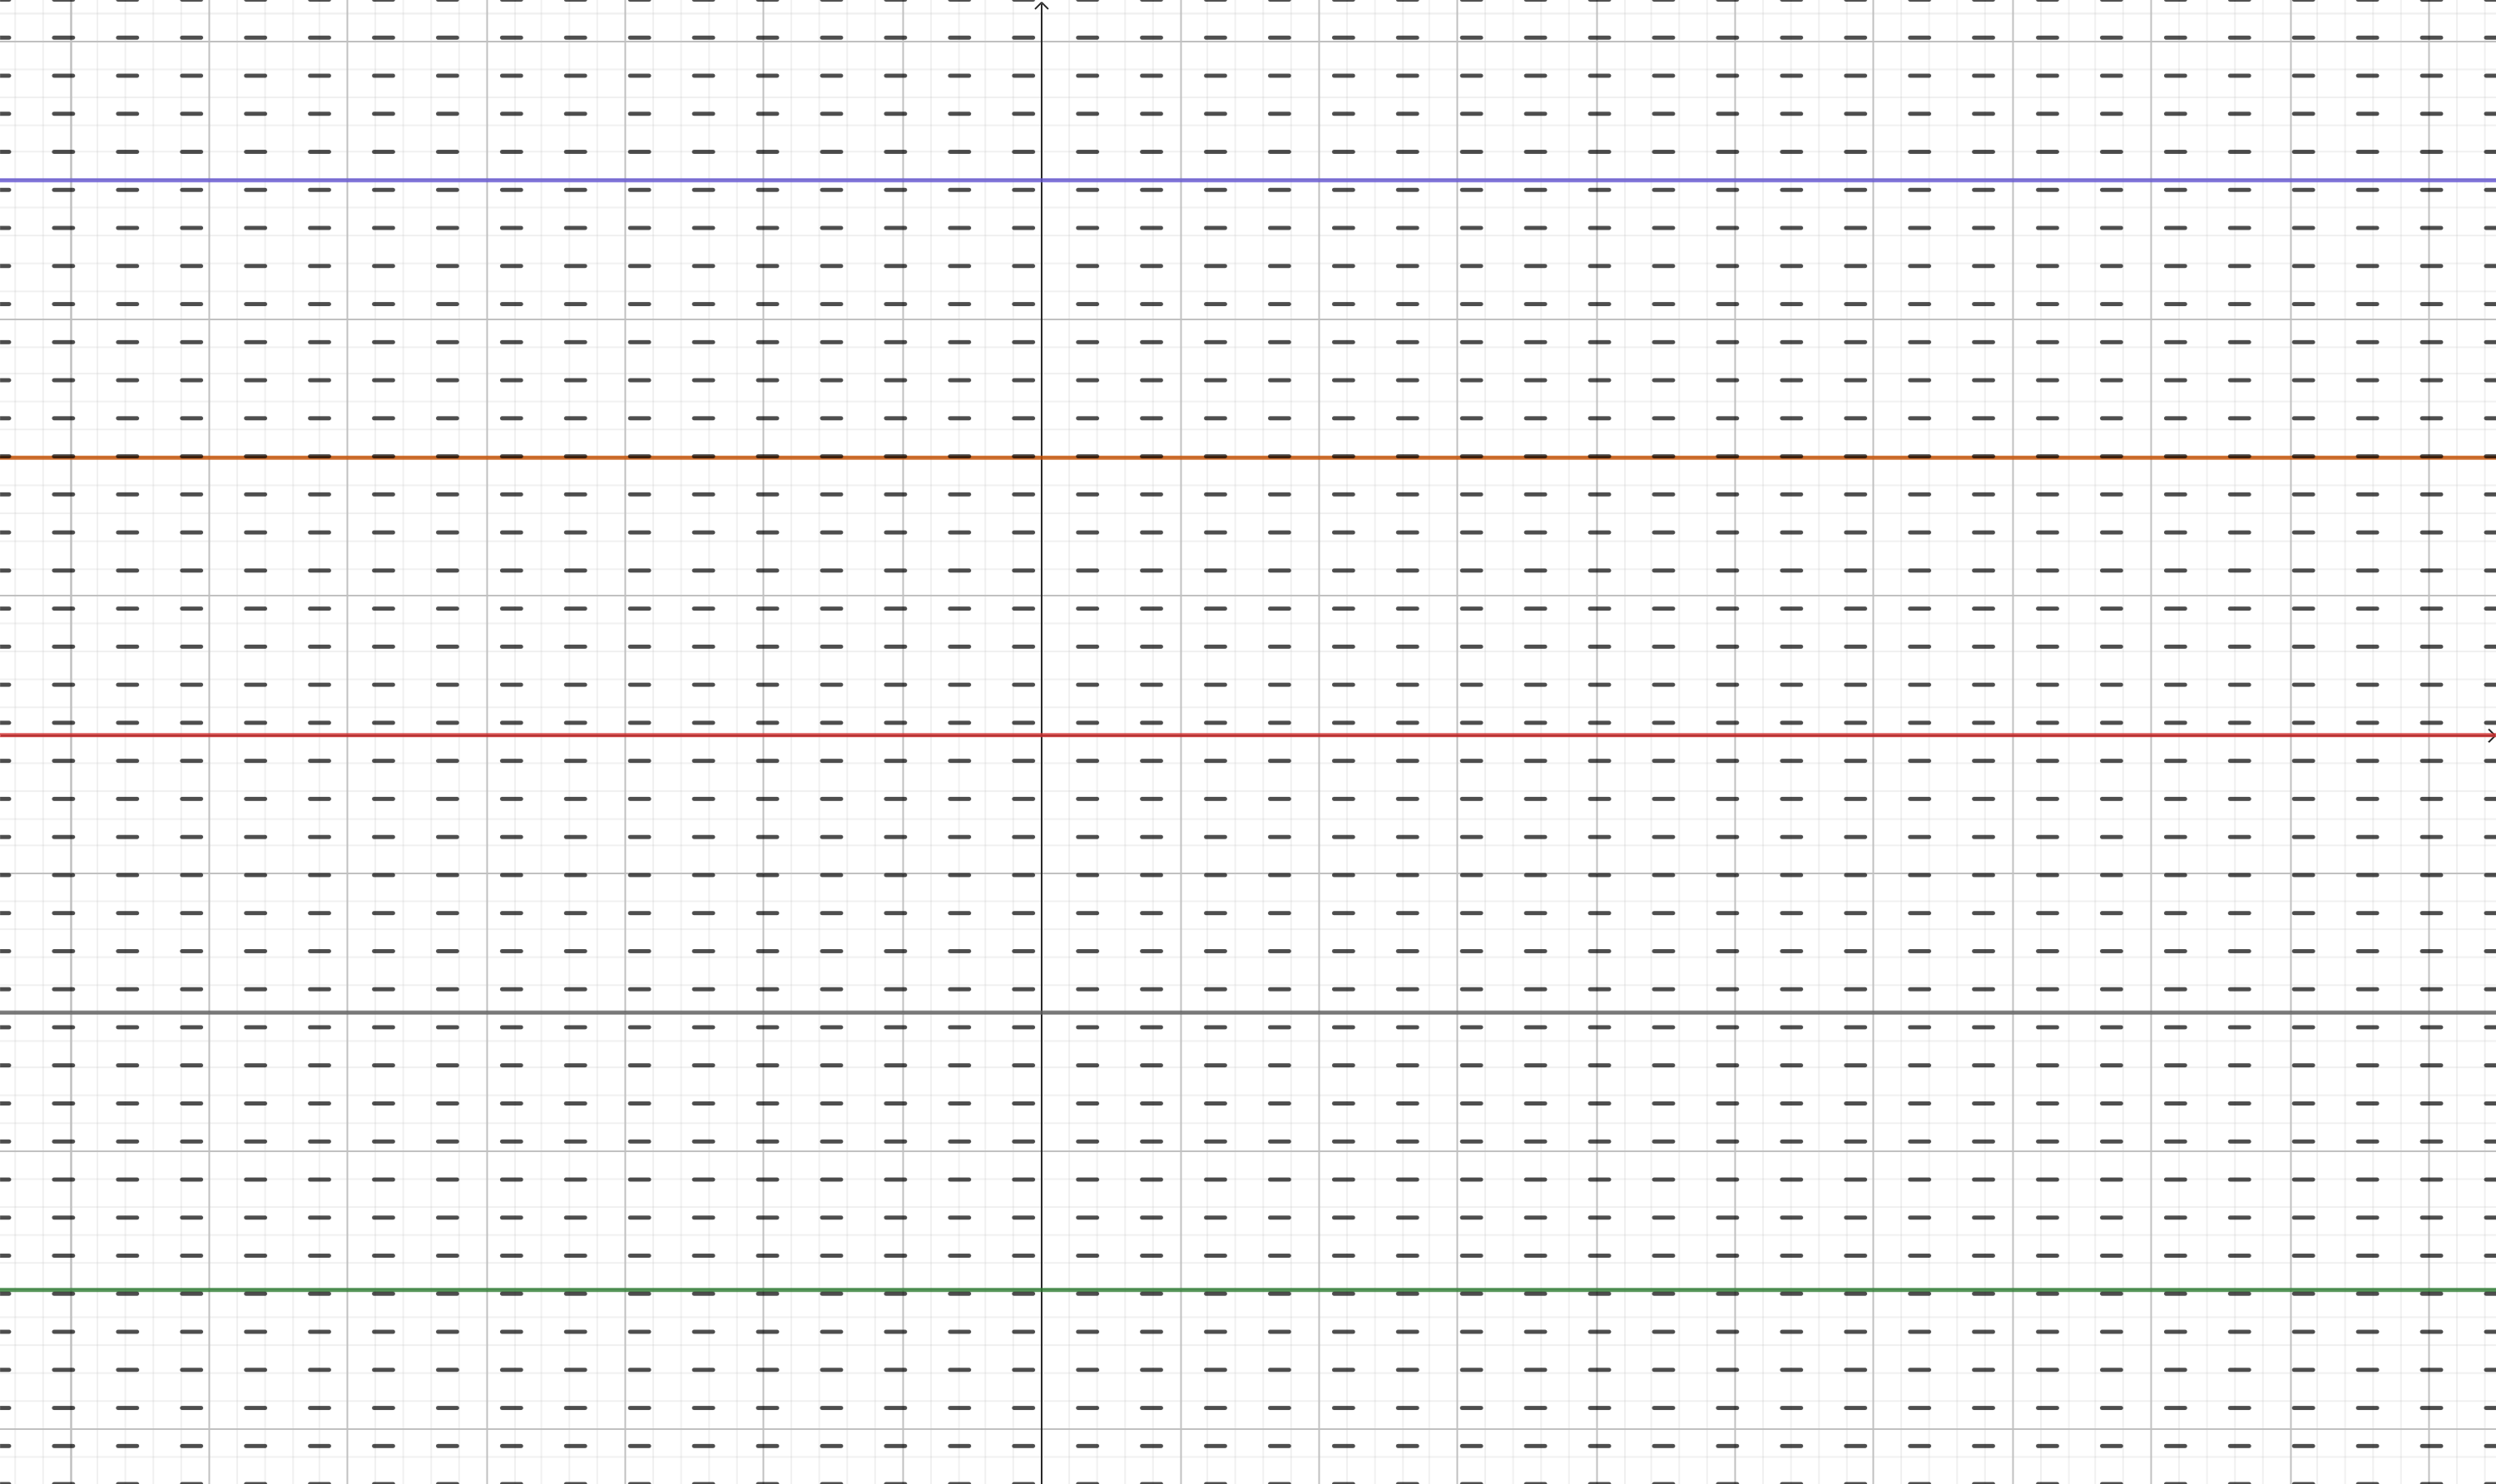
\includegraphics[width=0.6\linewidth]{Imagenes/campo_direcciones_1.png}
        \caption{Campo de direcciones para $x'=0$ y algunas soluciones de la misma.}
    \end{figure}
\fi
\end{ejemplo}

\begin{ejemplo}
    Consideremos ahora:
    \begin{equation*}
        x' = 1
    \end{equation*}
    Cuyas soluciones son de la forma:
    \begin{equation*}
        x(t) = x + c \quad c\in \mathbb{R}, \quad t\in \mathbb{R}
    \end{equation*}
    En este caso, el campo de direcciones viene dado por
    \Func{f}{\mathbb{R}^2}{\mathbb{R}}{(t,x)}{1}
    por lo que a cada punto $(t,x)$ le asociamos una recta a 45º de inclinación.

\ifdefined\showimages
    \begin{figure}[H]
        \centering
        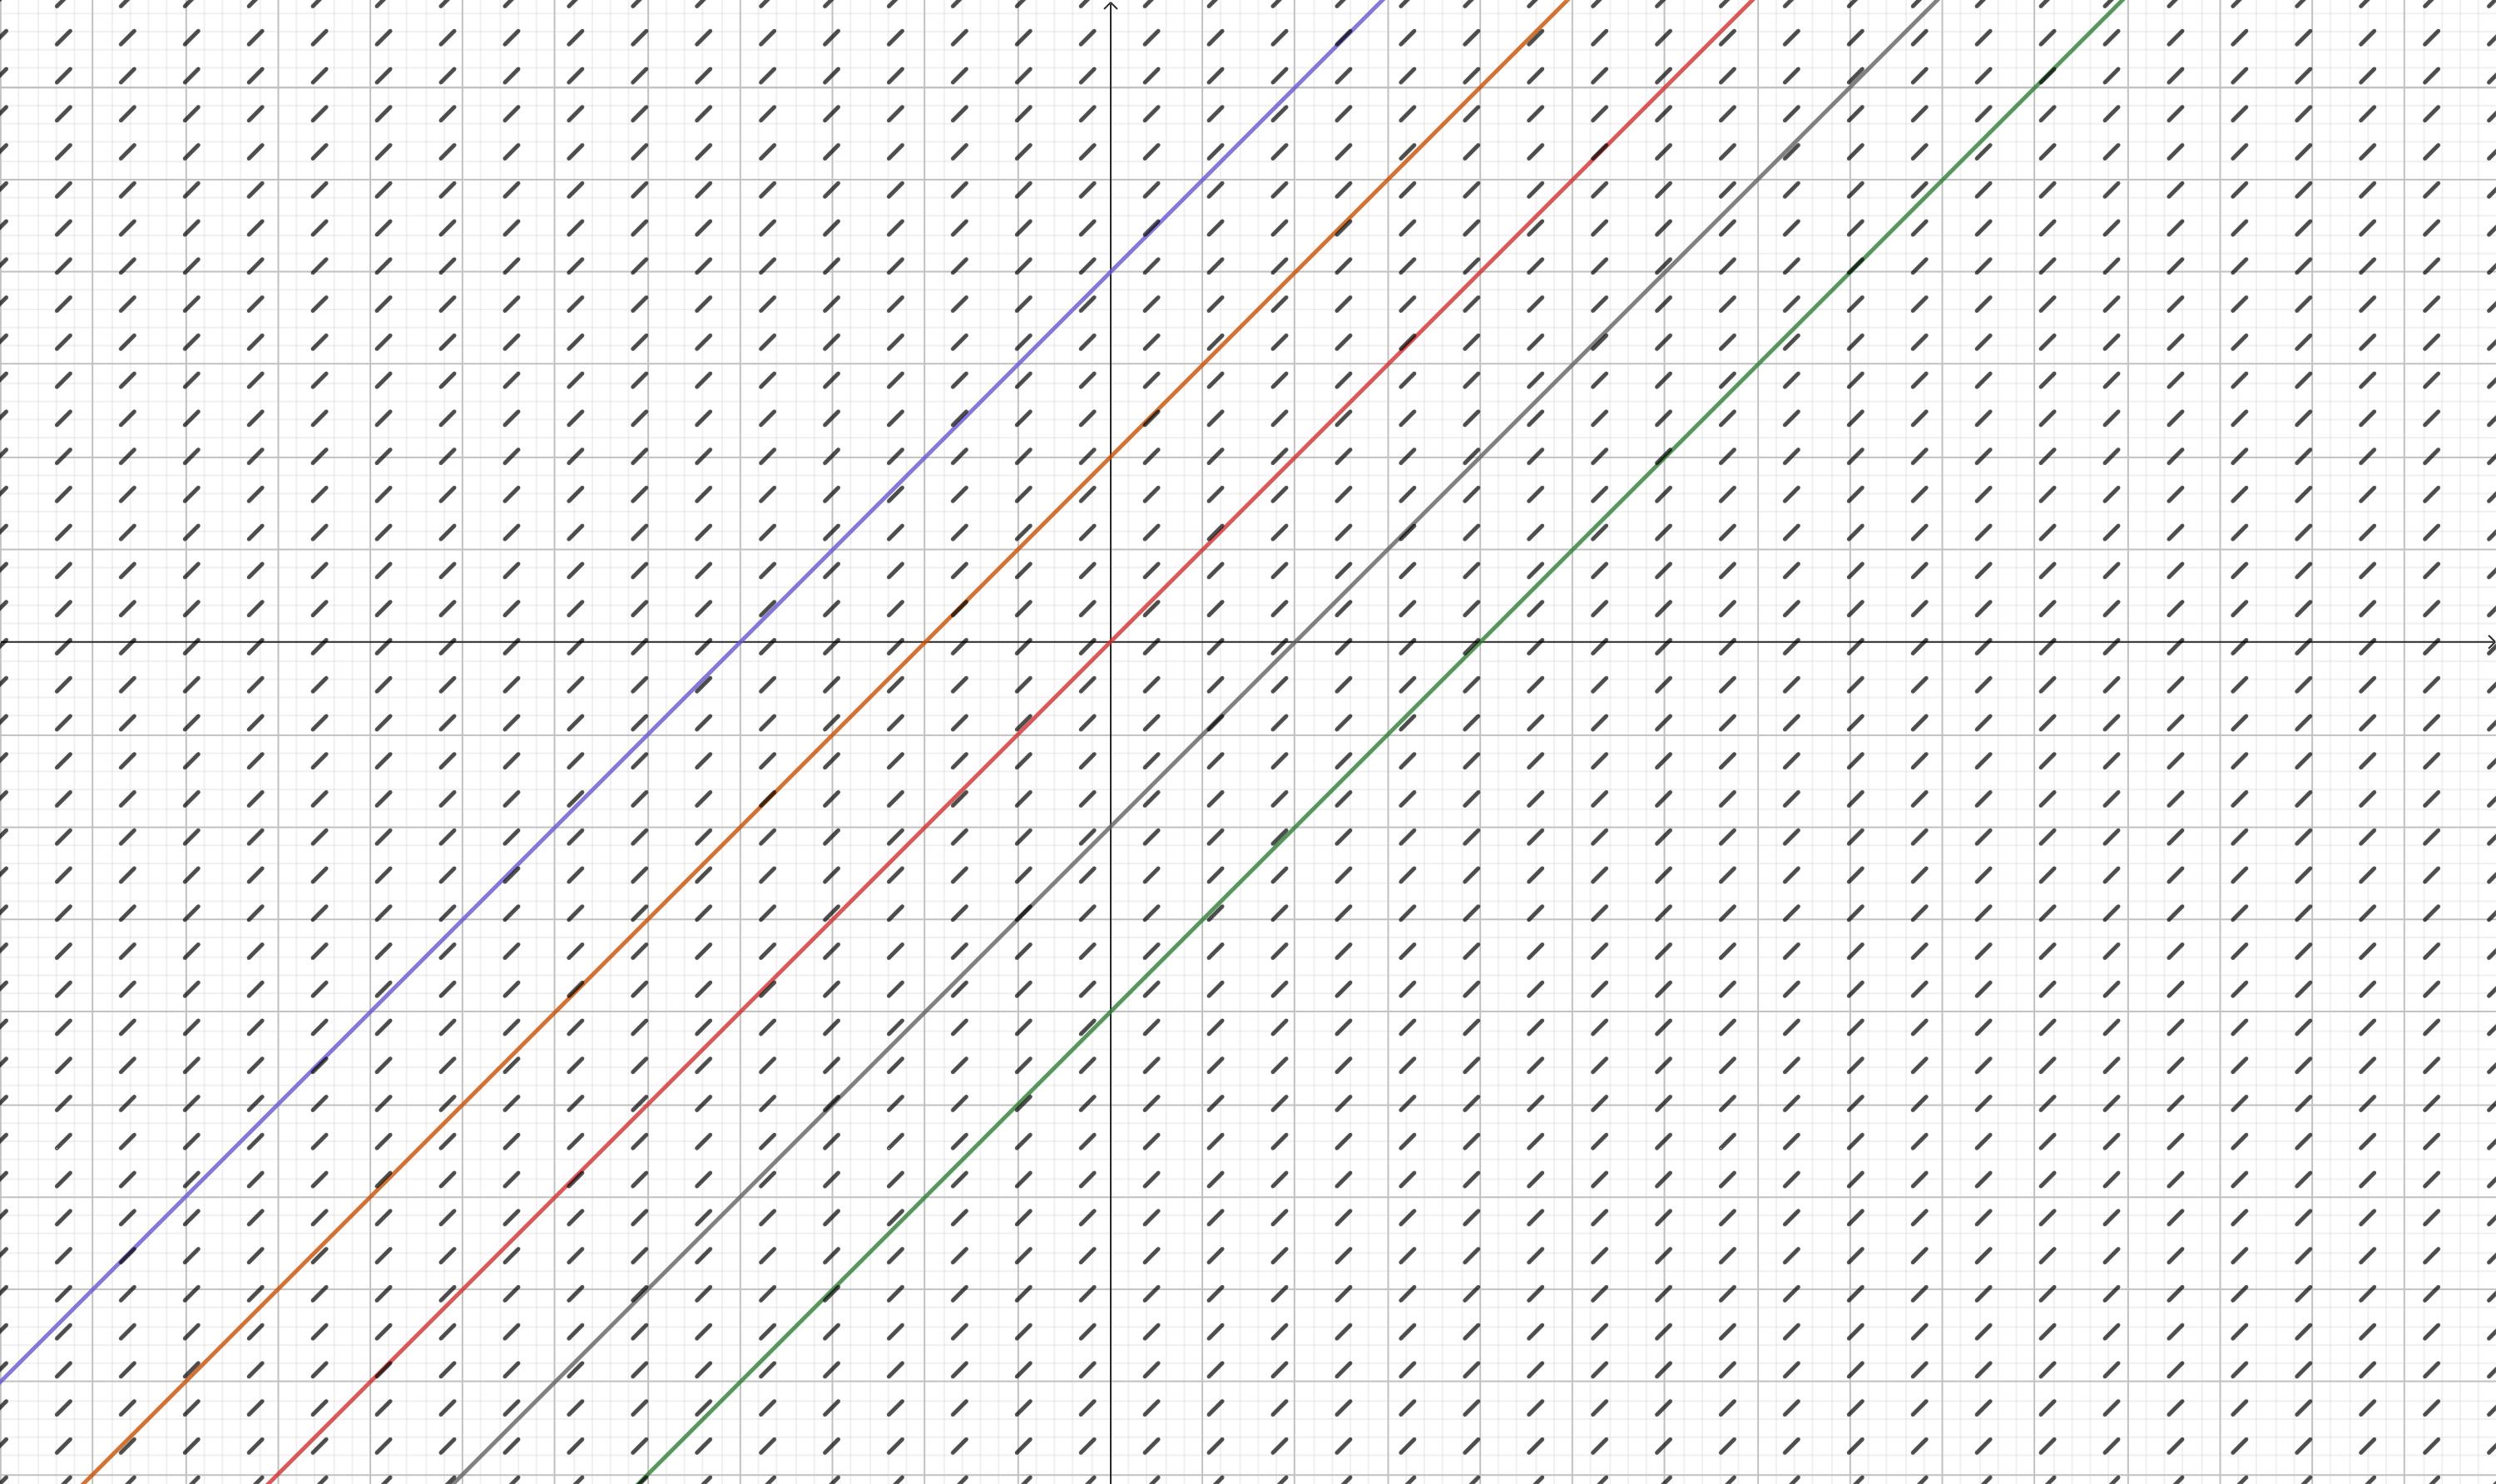
\includegraphics[width=0.6\linewidth]{Imagenes/campo_direcciones_2.png}
        \caption{Campo de direcciones para $x'=1$ y algunas soluciones de la misma.}
    \end{figure}
\fi
\end{ejemplo}

\begin{ejemplo}
    Consideramos:
    \begin{equation*}
        x'=x
    \end{equation*}
    Cuyas soluciones sabemos que son:
    \begin{equation*}
        x(t) = c\cdot e^{t} \quad c\in \mathbb{R}, \quad t\in \mathbb{R}
    \end{equation*}
    Ahora, la función que nos da el campo de direcciones es
    \Func{f}{\mathbb{R}^2}{\mathbb{R}}{(t,x)}{x}
    Para pensar en el campo de direcciones, pensemos en ir dibujándolo por cada recta horizontal del plano:
    \begin{itemize}
        \item Para puntos $(t,x)$ de la recta $x=0$, tendremos $f(t,x) = 0$, luego para todos los puntos del eje de abscisas tenemos siempre rectas horizontales.
        \item Para los puntos de la recta $x=1$, tendremos rectas a 45º de inclinación.
        \item Para $x=-1$, tendremos rectas a -45º de inclinación.
        \item De igual forma, para la recta $x=2$, tendremos rectas más inclinadas que la de 45º.
        \item De forma análoga, para los puntos de la recta $x=-2$, tendremos rectas más inclinadas que la de -45º.
    \end{itemize}
    En definitiva, cuanto más nos alejamos del eje de abscisas, más pendientes se ponen las rectas del campo de direcciones.

\ifdefined\showimages
    \begin{figure}[H]
        \centering
        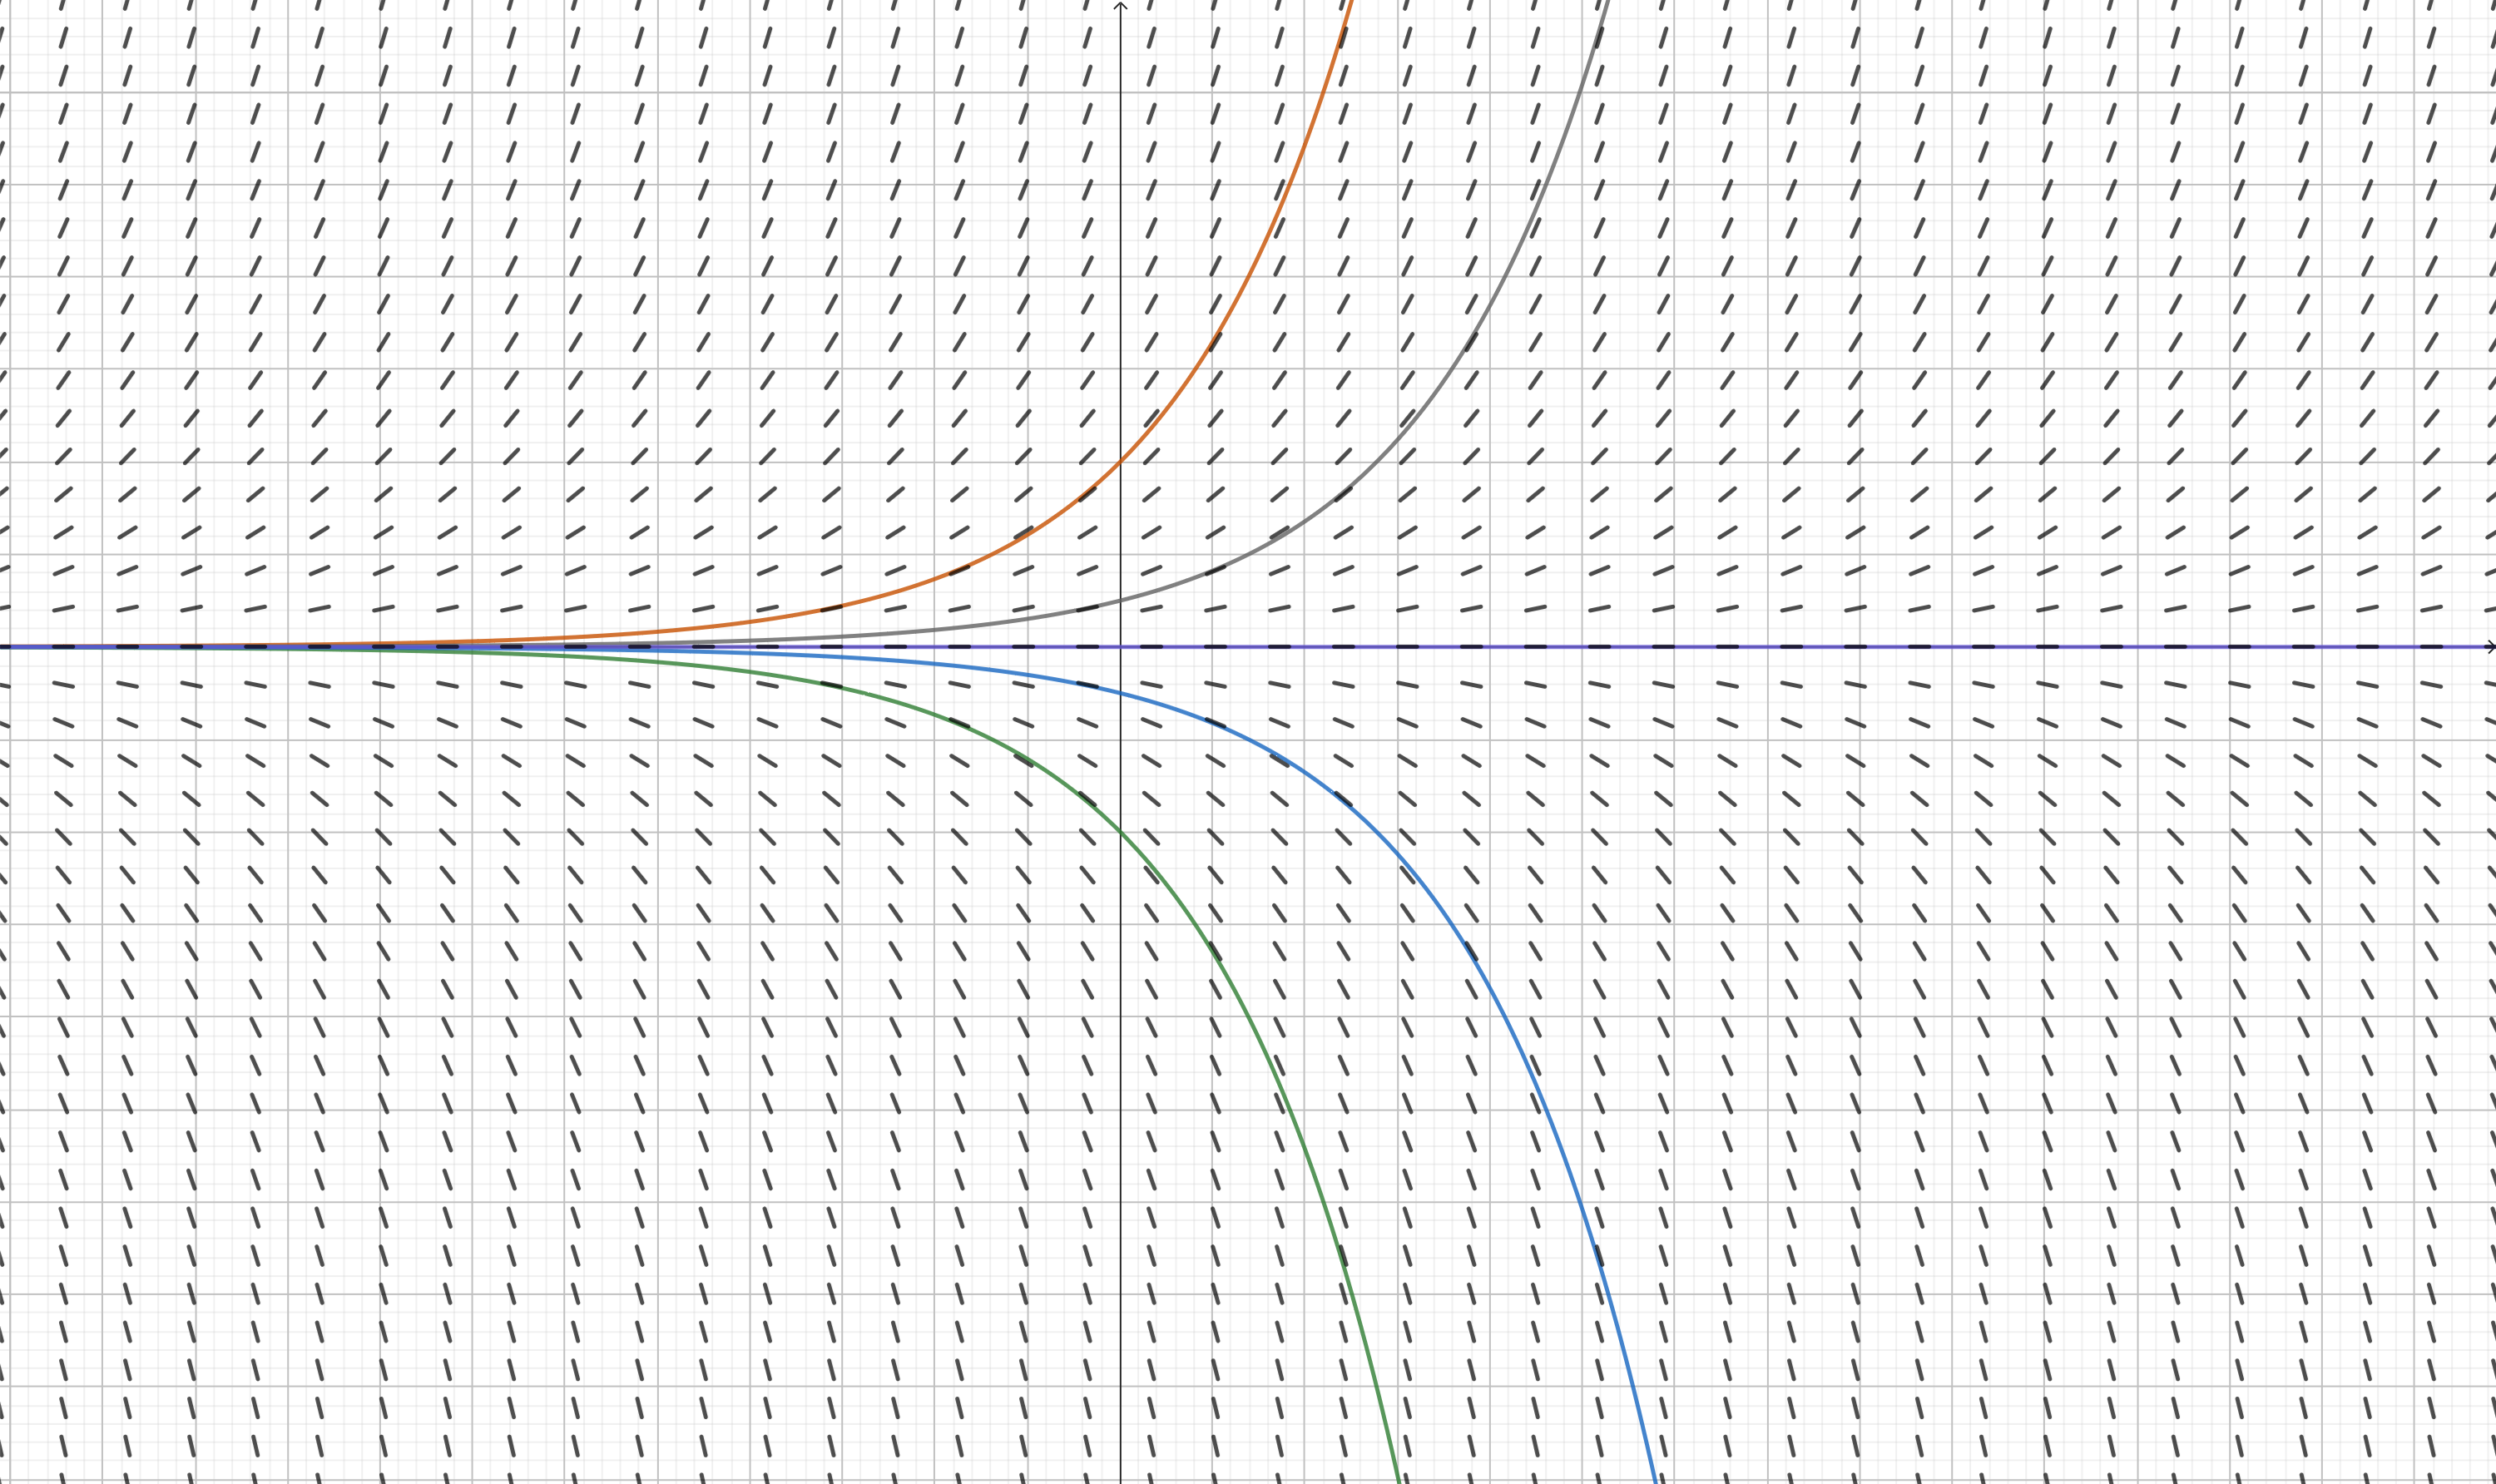
\includegraphics[width=0.6\linewidth]{Imagenes/campo_direcciones_3.png}
        \caption{Campo de direcciones para $x'=x$ y algunas soluciones de la misma.}
    \end{figure}
\fi
\end{ejemplo}

\begin{ejemplo}
    Consideramos:
    \begin{equation*}
        x' = t^2 + x^2
    \end{equation*}
    Cuyas soluciones se han demostrado (no se verá) que no tienen fórmula que pueda escribirse con funciones elementales clásicas.

    Pese a ello, sabemos que la función que nos da su campo de direcciones es:
    \Func{f}{\mathbb{R}^2}{\mathbb{R}}{(t,x)}{t^2+x^2}
    Para visualizar el campo de direcciones, pensaremos en circunferencias centradas en el origen con distinto radio $r\in \mathbb{R}^+_0$:
    \begin{itemize}
        \item Para $r = 0$, tenemos la circunferencia formada por el punto $(0,0)$, con $f(0,0) = 0$, luego tenemos que la recta asociada a dicho punto es una recta horizontal.
        \item Para $r = 1$, tenemos que $t^2 + x^2 = r^2 = 1$ para cada punto $(t,x)$ de dicha circunferencia, luego tenemos una recta a 45º de inclinación en cada punto de dicha circunferencia.
        \item Para $r = 2$, tenemos que $t^2 + x^2 = r^2 = 4$ para cada punto de la circunferencia, luego tendríamos una recta de mayor inclinación en dichos puntos.
    \end{itemize}
    Podemos ya imaginarnos cuál será el campo de direcciones, el cual podemos graficar gracias a los ordenadores:
\ifdefined\showimages
    \begin{figure}[H]
        \centering
        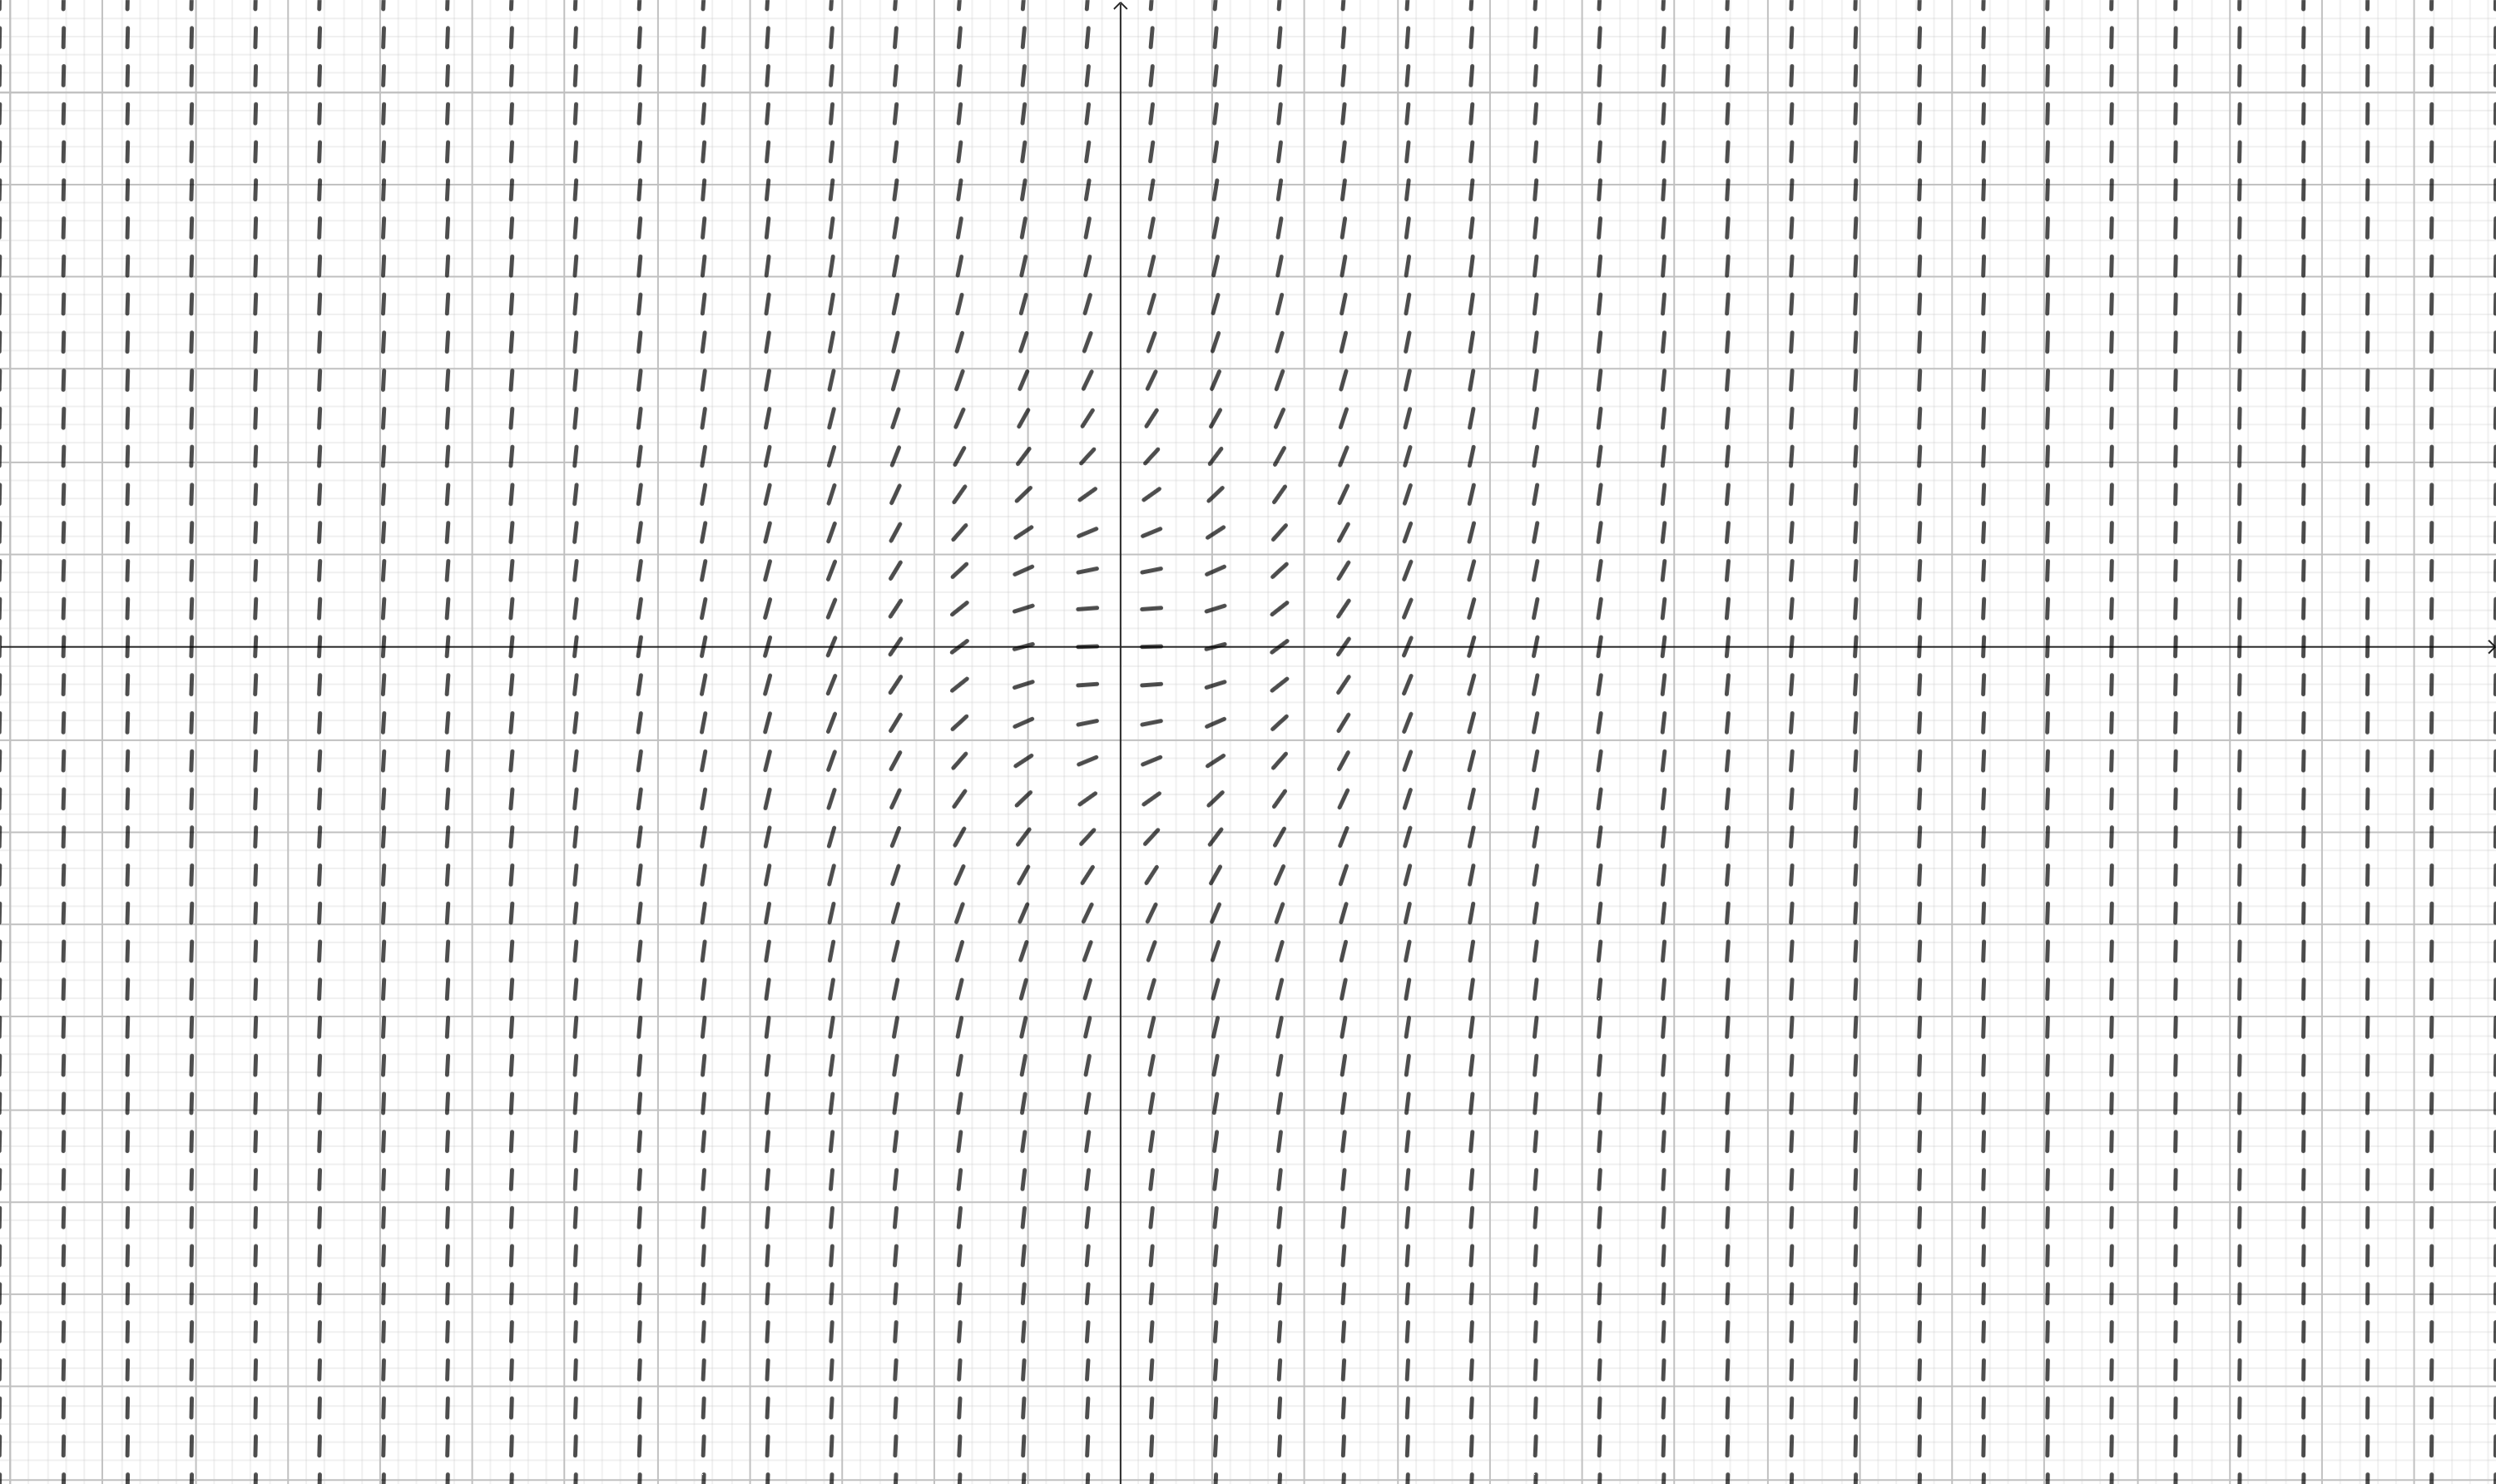
\includegraphics[width=0.6\linewidth]{Imagenes/campo_direcciones_4.png}
        \caption{Campo de direcciones para $x'=t^2+x^2$.}
    \end{figure}
\fi
    No conocemos soluciones para esta ecuación diferencial. Sin embargo, observando el campo de direcciones, observamos que las soluciones son funciones crecientes, con límite a $-\infty$ por la izquierda y a $+\infty$ por la derecha.
\end{ejemplo}

\section{Funciones implícitas}
Hasta ahora, hemos trabajado principalmente con funciones definidas en forma explícita $x=x(t)$. Sin embargo, en ecuaciones diferenciales es común trabajar con funciones definidas por una ecuación de la forma
\begin{equation*}
    F(t,x) = 0
\end{equation*}
por lo que tenemos que saber trabajar con ellas.\\

Cabe destacar que toda función explícita puede ponerse como implícita, pero no toda función implícita dada por una fórmula puede ponerse como función explícita. De esta forma, el estudio que realizaremos a continuación está enfocado a dichas funciones implícitas que no pueden ponerse de forma explícita.

Por lo tanto, si nos encontramos con una ecuación que nos da una función implícita de la cual podemos despejar $x$, podemos expresar la función de forma explícita y no será necesario aplicar lo aprendido en esta sección.

\begin{ejemplo}
    La fórmula
    \begin{equation*}
        x-t = 0
    \end{equation*}
    nos define una ecuación implícita $x=x(t)$, ya que dado un $t\in \mathbb{R}$, existe un único $x\in \mathbb{R}$ tal que se verifica la fórmula. Sin embargo, dicha función $x$ podemos expresarla de forma explícita, sacando su fórmula despejando $x$ de la fórmula anterior:
    \begin{equation*}
        x(t) = t \quad \forall t\in \mathbb{R}
    \end{equation*}
    Y podremos trabar con ella como una función explícita, algo a lo que ya estamos acostumbrados.
\end{ejemplo}

\begin{ejemplo}
    Veamos que la fórmula
    \begin{equation}\label{eq:ejm1}
        x^7+3x+t^2 = 0
    \end{equation}
    nos define una función implícita $x(t)$, es decir, que dado un número $t\in \mathbb{R}$, existe un único valor $x\in \mathbb{R}$ que verifique la fórmula~(\ref{eq:ejm1}).\\

    Dado $t\in \mathbb{R}$, hemos de probar la existencia y unicidad de $x\in \mathbb{R}$ tal que verifique la fórmula~(\ref{eq:ejm1}). Cuando lo tengamos probado, notaremos $x(t) = x$ para dicho $t$ y tendremos probado que la fórmula~(\ref{eq:ejm1}) nos define una función implícita.
    \begin{proof}~\\
        \begin{description}
            \item [Existencia.]~\\
                Dado $t\in \mathbb{R}$, podemos definir el polinomio
                \begin{equation*}
                    p_t(x) = x^7+3x+t^2
                \end{equation*}
                Y por ser un polinomio de grado impar, conocemos que al menos tiene una raíz $x\in \mathbb{R}$ tal que se verifica la fórmula~(\ref{eq:ejm1})\footnote{Es contenido de Álgebra I, pero puede deducirse ya que tiene límite a $-\infty$ por la izquierda y a $+\infty$ por la derecha, y aplicamos el Teorema de Bolzano.}.\\
            \item [Unicidad.]~\\
                Derivamos ahora el polinomio $p_t$:
                \begin{equation*}
                    p_t'(x) = 7x^6+3 > 0 \quad \forall x\in \mathbb{R}
                \end{equation*}
                Luego es una función estrictamente creciente, por lo que a lo sumo tiene una raíz.
        \end{description}
    \end{proof}
\end{ejemplo}

Acabamos de ver un ejemplo de fórmula que nos define una única función implícita $x=x(t)$.  Nos preguntamos a continuación si cualquier fórmula nos provee de una función implícita. En caso de hacerlo, ¿obtenemos funciones derivables? Dicha pregunta nos servirá de paso para probar que la función implícita $x=x(t)$ del ejempmlo anterior es derivable.\\

\begin{enumerate}
    \item Como primera observación sencilla, mostramos que hay ecuaciones que no nos definen ninguna función implícita, como:
        \begin{equation*}
            x^2+t^2 = -1
        \end{equation*}
        Ya que dado $t\in \mathbb{R}$ no podemos encontrar ningún $x\in \mathbb{R}$ tal que se verifique la ecuación.

    \item Además, hay ecuaciones que nos dan más de una función implícita, como el clásico ejemplo de la circunferencia:
        \begin{equation*}
            x^2 + t^2 = 1
        \end{equation*}
        Dicha ecuación nos fabrica dos funciones implícitas que además podemos expresar de forma explícita:
        \begin{align*}
            x_1(t) &= +\sqrt{1-t^2}, \quad t\in [-1,1] \\
            x_2(t) &= -\sqrt{1-t^2}, \quad t\in [-1,1] \\
        \end{align*}

    \item Finalmente, observamos que hay funciones implícitas que no se pueden derivar. Por ejemplo, la fórmula:
        \begin{equation*}
            x^3-t^2 = 0
        \end{equation*}
        nos da una función implícita que podemos poner como explícita:
        \begin{equation*}
            x(t) = t^{\nicefrac{2}{3}}, \quad t\in \mathbb{R}
        \end{equation*}
        Pero dicha función no es derivable en 0.
\end{enumerate}

En resumen, dada una fórmula que nos relacione dos variables:
\begin{equation*}
    F(t,x) = 0
\end{equation*}
no podemos asegurar que la función implícita que nos da (en caso de hacerlo) sea derivable, puede pasar cualquier cosa: a veces no define ecuación implícita, a veces define varias, puede definirnos sólo una que no sea derivable, o que sí lo sea, \ldots No contamos con una teoría general de ecuaciones implícitas.\\

Sin embargo, contamos con un resultado bastante útil que ya conocimos en Análisis Matemático I, el Teorema de la Función Implícita\footnote{Aunque en Análisis Matemático I se dió el teorema en su forma más general, en esta asignatura nos interesará el caso de $\mathbb{R}^2$.}. Se trata de un teorema local que da condiciones para que exista la función implícita y sea única, dentro de un entornon suficientemente pequeño.

\begin{teo}[Función Implícita]
    Sea $G\subseteq \mathbb{R}^2$ un abierto y sea
    \Func{F}{G}{\mathbb{R}}{(t,x)}{F(t,x)}
    una función de clase $\mathcal{C}^1(\mathbb{R}^2)$, es decir, que existan las parciales respecto a $t$ y respecto a $x$ y que ambas sean continuas.

    \noindent
    Sea $(t_0,x_0)\in G$ de forma que $F(t_0,x_0)=0$ y se cumpla que:
    \begin{equation*}
        \dfrac{\partial F}{\partial x}(t_0,x_0) \neq 0
    \end{equation*}
    Entonces, existe una función 
    \Func{x}{I}{\mathbb{R}}{t}{x(t)}
    con $I\subseteq \mathbb{R}$ un intervalo abierto de forma que $x\in \mathcal{C}^1(I)$ y se verifica:
    \begin{enumerate}
        \item $t_0 \in I$.
        \item $x(t_0) = x_0$.
        \item $(t,x(t))\in G$ $\forall t\in I$.
        \item $F(t,x(t))=0$ $\forall t\in I$.
    \end{enumerate}
\end{teo}~\\

% // TODO: Borrar cuando sepa fijo que está bien el teorema
%El dominio $G$ tiene que ser un abierto y la función $F$ ha de ser una función de clase $C^1(G)$. Es decir, que existan las parciales respecto a $t$ y respecto a $x$ y que ambas sean continuas. 
%
%Como el teorema es local, necesitamos un punto $(t_0,x_0)\in G$ en el que estudiar la función, luego se cumplirá la ecuación $F(t_0,x_0)=0$. Además, tenemos que obligar a que la parcial respecto a la variable que queremos hacer dependiente no se anule: $\dfrac{\partial F(t,x)}{\partial x} \neq 0$.
%
%En dicho caso, $\exists x:I\rightarrow\mathbb{R}$ con $I$ un intervalo abierto de forma que $t_0\in I$ tal que $x(t_0) = x_0$, $x\in C^1(I)$, se cumple que $(t,x(t)) \in G$ $\forall t\in I$ y que $F(t,x(t)) = 0$ $\forall t\in I$

Veremos ahora varios usos prácticos del teorema:
\begin{ejemplo}
    En el caso
    \begin{equation*}
        x^2+t^2 = 1
    \end{equation*}
    Tenemos la función 
    \Func{F}{\mathbb{R}^2}{\mathbb{R}}{(t,x)}{x^2 + t^2 - 1}
    que es de clase $C^1(\mathbb{R}^2)$:
    \begin{equation*}
        \dfrac{\partial F}{\partial t}(t,x) = 2t \qquad \dfrac{\partial F}{\partial x}(t,x) = 2x \qquad \forall (t,x)\in \mathbb{R}^2
    \end{equation*}
    Buscamos ahora un punto $(t_0,x_0)\in \mathbb{R}^2$ para aplicar el teorema:
    \begin{itemize}
        \item Ha de ser un punto de la circunferencia de radio 1, para que $F(t_0,x_0)=0$.
        \item Además, ha de ser $x_0 \neq 0$, para que:
            \begin{equation*}
                \dfrac{\partial F}{\partial x}(t_0,x_0) = 2x_0 \neq 0
            \end{equation*}
    \end{itemize}
    De esta forma, podemos elegir cualquier punto $(t_0,x_0)\in \mathbb{S}^1\setminus \{(-1,0),(1,0)\}$ para aplicar el teorema.

    Por tanto, dado cualquier punto $t_0\in \left]-1,1\right[$, el teorema nos dice que hay un intervalo abierto $I$ de forma que $t_0\in I \subseteq \left]-1,1\right[$ en el que la función (ya sea la anterior $x_1$ o $x_2$) es derivable.\\

    Sabíamos ya de antemano la existencia de dichas funciones, pero en caso de no saberlo el Teorema nos garantiza dicha existencia. Este es el primer uso del teorema.
\end{ejemplo}

\begin{ejemplo}
    En el caso:
    \begin{equation*}
        x^7+3x+t^2 = 0
    \end{equation*}
    ya sabemos que existe la función implícita, pero no sabemos si dicha función es derivable o no. Usaremos el Teorema de la función implícita para probar que la función $x=x(t)$ que nos da la fórmula es derivable:

    \noindent
    Sea $G = \mathbb{R}^2$ y $F(t,x) = x^7+3x+t^2$ que es una función de clase $\mathcal{C}^1(\mathbb{R}^2)$:
    \begin{equation*}
        \dfrac{\partial F}{\partial t}(t,x) = 2t \qquad \dfrac{\partial F}{\partial x}(t,x) = 7x^6 + 3 \qquad \forall (t,x)\in \mathbb{R}^2
    \end{equation*}
    Notemos que:
    \begin{equation*}
        \dfrac{\partial F}{\partial x}(t,x) = 7x^6 + 3 > 0
    \end{equation*}
    Por lo que podemos elegir cualquier punto en el que $F(t,x) = 0$ para aplicar el teorema, obteniendo que la función $x$ es derivable.\\

    Este es el segundo uso práctico del teorema, probar de forma fácil que una función implícita que ya conocemos es derivable.
\end{ejemplo}

\begin{ejemplo}
    Anteriormente, vimos que la fórmula
    \begin{equation*}
        x^3-t^2 = 0
    \end{equation*}
    que define una función implícita:
    \begin{equation*}
        x(t) = t^{\nicefrac{2}{3}}, \quad t\in \mathbb{R}
    \end{equation*}
    no era derivable. Comprobamos qué hipótesis es la que falla del teorema:

    \noindent
    Tenemos
    \Func{F}{\mathbb{R}^2}{\mathbb{R}}{(t,x)}{x^3-t^2}
    con parciales:
    \begin{equation*}
        \dfrac{\partial F}{\partial t}(t,x) = 2t \qquad \dfrac{\partial F}{\partial x}(t,x) = 3x^2 \qquad \forall (t,x)\in \mathbb{R}^2
    \end{equation*}
    luego $F\in \mathcal{C}^1(\mathbb{R}^2)$. En el ejemplo anterior, fallaba la derivabilidad en $t_0 = 0$, luego comprobamos por qué la función no es derivable:

    \noindent
    En primer lugar, para tener que $x_0^3 - t_0^2 = 0$ con $t_0 = 0$ ha de ser $x_0 = 0$. Sin embargo:
    \begin{equation*}
        \dfrac{\partial F}{\partial x}(0,0) = 0
    \end{equation*}
    Luego no podemos aplicar el teorema de la Función Implícita.
\end{ejemplo}

\subsection{Derivación implícita}
Hasta ahora, tenemos una forma de probar la existencia de funciones implícitas así como su derivabilidad, pero no sabemos cómo derivarlas, lo cual trataremos de resolver a continuación.\\

\noindent
Usualmente, tendremos una función
\Func{F}{G\subseteq \mathbb{R}^2}{\mathbb{R}}{(t,x)}{F(t,x)}
de clase $\mathcal{C}^1(\mathbb{R}^2)$ que verifique las hipótesis del Teorema de la Función Implícita, de forma que:
\begin{equation}\label{eq:formula_deriv_implicita}
    F(t,x(t)) = 0 \quad \forall t\in I
\end{equation}
para cierta función $x=x(t)$ e $I\subseteq \mathbb{R}$ intervalo abierto. Nuestro objetivo será derivar la expresión anterior.

\begin{prop}
    Dadas unas funciones $F$ como la definida anteriormente, $x$ y $t$ funciones reales de variable real de clase $\mathcal{C}^1(\mathbb{R})$ y una función como resultado de la composición de funciones:
    \begin{equation*}
        s \longmapsto (t(s), x(s)) \longmapsto F(t(s), x(s))
    \end{equation*}
    que es también una función real de variable real de clase $\mathcal{C}^1(\mathbb{R})$, tenemos que:
    \begin{equation*}
        \dfrac{d}{ds}[ F(t(s),x(s))] = \dfrac{\partial F}{\partial t}(t(s), x(s))\cdot t'(s) + \dfrac{\partial F}{\partial x}(t(s),x(s))\cdot x'(s) \quad \forall s\in \mathbb{R}
    \end{equation*}
\end{prop}~\\

\noindent
Usando esta proposición sobre la fórmula~(\ref{eq:formula_deriv_implicita}), llegamos a la ecuación diferencial:
\begin{equation*}
    \dfrac{dF}{dt}(t,x(t)) = \dfrac{\partial F}{\partial t}(t,x(t)) + \dfrac{\partial F}{\partial x}(t,x(t))\cdot x'(t) = 0
\end{equation*}
Que no se encuentra en forma normal. Sin embargo, es usual haber aplicado el Teorema de la Función Implícita antes de este resultado, luego, suponiendo que estamos bajo dichas hipótesis, tendremos que 
\begin{equation*}
    \dfrac{\partial F}{\partial x}(t,x(t)) \neq 0
\end{equation*}
en un entorno de $t$, por lo que en dicho caso sí que podremos despejar la ecuación diferencial anterior, para expresarla en forma normal:
\begin{equation*}
    x'(t) = \dfrac{-\dfrac{\partial F}{\partial t}(t,x(t))}{\dfrac{\partial F}{\partial x}(t,x(t))}
\end{equation*}

\section{Ecuación diferencial a partir de una familia de funciones}
Al igual que sucede con los polinomios y sus raíces, es mucho más simple construir una ecuación diferencial a partir de una familia de soluciones a obtener la familia de funciones que resuelve una ecuación diferencial.\\

En esta sección, nos centraremos en cómo construir una ecuación diferencial de primer orden a partir de una familia uniparamétrica de funciones implícitas.

Para ello, nos darán una ecuación del tipo:
\begin{equation*}
    F(t,x,c) = 0
\end{equation*}

siendo $c$ el parámetro, y definiéndonos una familia de funciones implícitas, de donde obtenemos la función implícita $x=x(t)$, y llegamos a:

\begin{equation*}
    F(t,x(t),c) = 0
\end{equation*}

y lo que haremos para obtener la ecuación diferencial es derivar:
\begin{equation*}
    \dfrac{dF}{dt}(t,x(t),c) = \dfrac{\partial F}{\partial t}(t,x(t),c) + \dfrac{\partial F}{\partial x}(t,x(t),c)\cdot x'(t) = 0
\end{equation*}
Que no es una ecuación diferencial, sino una familia de ecuaciones diferenciales, ya que para cada $c\in \mathbb{R}$ tenemos una ecuación diferencial distinta.

El último paso, por tanto, es tratar de expresar $c$ en función de $x$ y de $t$, para sustituirlo y obtener finalmente la ecuación diferencial:

\begin{equation*}
    \left.\begin{array}{rr}
                F(t,x(t),c) &= 0 \\
                \dfrac{\partial F}{\partial t}(t,x(t),c) + \dfrac{\partial F}{\partial x}(t,x(t),c)\cdot x'(t) &= 0
        \end{array}\right\} \overset{\text{Despejar $c$}}{\longrightarrow } \Phi(t,x,x') = 0
\end{equation*}
No es necesario hacer este proceso de forma rigurosa, ya que lo único que nos pedirán es obtener una ecuación difrencial que tenga por soluciones la familia uniparamétrica de funciones dada. Por tanto, siempre y cuando que consigamos este objetivo, podemos responder a la pregunta simplemente dando la ecuación diferencial y probando que, efectivamente, dicha familia es solución de la ecuación.

\begin{ejemplo}
    Hallar la ecuación diferencial que tiene por soluciones la familia uniparamétrica de funciones:
    \begin{equation}\label{eq:ejm1_ecuacion_familia}
        x^2+t^2 = c\qquad c\in \mathbb{R}^+
    \end{equation}
    En primer lugar, ya sabemos que dicha fórmula nos da una familia uniparamétrica de funciones:
    \begin{equation*}
        x(t) = \pm \sqrt{c-t^2}, \quad t\in \left]-c,c\right[
    \end{equation*}
    Tratamos ahora de hallar la ecuación diferencial que nos solicitan, que lo haremos derivando en ambos miembros de la fórmula~(\ref{eq:ejm1_ecuacion_familia}):
    \begin{align*}
        {(x(t))}^{2}+t^2 &= c \\
        \dfrac{d}{dt}\left({(x(t))}^{2}+t^2 \right) &= \dfrac{d}{dt}(c) \\
        2xx' + 2t &= 0
    \end{align*}
    En este caso, no ha sido necesario despejar $c$ para sustituirlo al final del cálculo anterior, ya que directamente ha desaparecido de la ecuación diferencial. De esta forma, la ecuación diferencial buscada es:
    \begin{equation*}
        2xx' + 2t = 0
    \end{equation*}
    Que podemos expresar en forma normal como:
    \begin{equation*}
        x' = \dfrac{-t}{x}
    \end{equation*}
\end{ejemplo}

\begin{observacion}
    Notemos que acabamos de aprender a resolver la ecuación diferencial
    \begin{equation*}
        x' = \dfrac{-t}{x}
    \end{equation*}
    Tiene por soluciones la familia uniparamétrica de funciones:
    \begin{equation*}
        x(t) = \pm \sqrt{c-t^2} \quad c\in \mathbb{R}^+, \quad t\in \left]-c,c\right[
    \end{equation*}
\end{observacion}


\begin{ejemplo}
    Buscar una ecuación diferencial que tenga como soluciones la familia uniparamétrica de funciones:
    \begin{equation}\label{eq:ejm2_ecuacion_familia}
        \dfrac{1}{c}e^{cx} - x^2 - \sen t = c
    \end{equation}
%     En primer lugar, comprobamos que, efectivamente, dicha fórmula nos da una familia uniparamétrica de funciones mediante el Teorema de la Función Implícita:\\
% 
%     Para cada $c\in \mathbb{R}^*$, definimos la función
%     \Func{F_c}{\mathbb{R}^2}{\mathbb{R}}{(t,x)}{\dfrac{1}{c} e^{cx}-x^2-\sen t -c}
% 
%     Con parciales:
%     \begin{equation*}
%         \dfrac{\partial F}{\partial t}(t,x) = -\cos t \qquad \dfrac{\partial F}{\partial x}(t,x) = e^{cx} -2x \qquad \forall (t,x) \in \mathbb{R}^2
%     \end{equation*}

    Tendríamos que $F(t,x,c) = \frac{1}{c}e^{cx} - x^2-\sen t - c$ y ahora derivaremos de forma implícita, pensando que la fórmula nos da una función $x=x(t)$:

    \begin{equation}\label{eq:ejm2_ecuacion_familia_2}
        \dfrac{d F}{d t}(t,x,c) = e^{cx}x' - 2x'x - \cos t = 0
    \end{equation}
    Ahora, nos disponemos a eliminar el parámetro $c$:

    Despejando en la fórmula~(\ref{eq:ejm2_ecuacion_familia_2}) llegamos a que:
    \begin{align*}
        e^{cx} &= \dfrac{2xx' + \cos t}{x'} \\
        cx &= \ln\left(\dfrac{2xx'+\cos t}{x'}\right) \\
        \dfrac{1}{c} &= \dfrac{x}{\ln \left(\dfrac{2xx' + \cos t}{x'}\right)}
    \end{align*}
    Y ahora sustituyendo $c$ y $\frac{1}{c}$ en~(\ref{eq:ejm2_ecuacion_familia}), tenemos que la ecuación diferencial buscada es:
    \begin{equation*}
       \dfrac{x}{\ln \left(\dfrac{2xx' + \cos t}{x'}\right)} \dfrac{2xx' + \cos t}{x'} - x^2-\sen t - \dfrac{1}{x}\ln \left(\dfrac{2xx' + \cos t}{x'}\right) = 0
    \end{equation*}
\end{ejemplo}

\section{Problemas geométricos relacionados con ecuaciones diferenciales}
Una aplicación de las ecuaciones diferenciales es hallar curvas exigiendo condiciones sobre sus tangentes o normales. Por ejemplo, podemos tratar de hallar la curva cuyas normales sean todas coincidentes en un mismo punto.

\begin{notacion}
    En esta sección haremos un cambio de notación, ya que las soluciones de las ecuaciones diferenciales ya no serán movimientos donde tratamos de expresar la posición $x$ de un móvil en función del tiempo $t$, $x = x(t)$; sino que las soluciones serán curvas geométricas, por lo que trataremos de, dada una abscisa $x$, hallar la coordenada en las ordenadas $y$ que nos diga un punto de la curva, $y = y(x)$.

    De esta forma, sustituiremos la notación que venimos usando de las ecuaciones diferenciales
    \begin{equation*}
        F(t,x) = 0
    \end{equation*}

    Por la notación
    \begin{equation*}
        F(x,y) = 0
    \end{equation*}
\end{notacion}

Aunque toda curva en el plano puede expresarse con una ecuación implícita (esto no sucede con explícitas), supondremos siempre que las curvas las podremos poner en explícitas, con la finalidad de que nos aparezcan siempre ecuaciones de primer orden (usando ecuaciones paramétricas, por ejemplo, obtenemos sistemas de ecuaciones).\\

De esta forma, trabajaremos con curvas $y=y(x)$ con $x\in I$ intervalo abierto, siendo $y\in \mathcal{C}^1(I)$\footnote{Con vistas para derivar y aplicar el Teorema de la Función Implícita.}.

\subsubsection{Rectas tangentes a una curva}
Sabemos ya que, dada una curva $y = y(x)$, podemos encontrar en cada punto $(x,y(x))$ una recta tangete a dicha curva. A medida que movemos el punto por la curva, vamos obteniendo todo el haz de rectas que son tangentes a dicha curva.\\

Dado un punto $(x,y(x))$ de una curva $y=y(x)$, la ecuación de la recta tangente a la curva en dicho punto viene dada por:
\begin{equation*}
    v-y(x) = y'(x) (u-x)
\end{equation*}
siendo $v$ y $u$ las nuevas variables que hemos usado para expresar la ecuación.\\

Dado $x\in \mathbb{R}$, el punto $(x,y(x))$ nos da una recta tangente a la curva por dicho punto. Si movemos la variable $u$, nos estaremos moviendo a lo largo de la recta tangete. Si ahora también movemos $x$, nos estaremos moviendo por todo el haz de rectas.

